
\begin{table*}[th]
\normalsize
\centering
\caption{The templates in the description generator. Placeholders are highlighted with a \textbf{\textit{bold italic}} font.}\label{tab:template}
\includegraphics[width=2\columnwidth]{figures/template.eps}
\vspace{-10pt}
\end{table*}

\section{Description Generator} \label{sec:generator}

\newfboxstyle{light-tight}{padding=1pt,margin=0pt,baseline-skip=false}
\fboxset{light-tight, rounded,border-style=dashed, border-radius=2pt,}%

We designed a set of templates to convert the encoded visual attributes into natural sentences (Figure~\ref{fig:workflow}b). The template is one of the most easy-to-understand ways to interpret visualization. Although many Natural Language Generation (NLG) techniques can generate more natural descriptions, the lack of training samples on node-link diagrams prevents them adapt to our scenarios. Moreover, the template is more controllable, which can be extended to different scenarios and keeps consistency.

\subsection{Description Template}

First, we present a sentence-level template by pre-setting several formats. Our template contains three parts -- 1) static texts, which bear a resemblance to the skeleton of the description and are basically consistent among different scenarios, 2) placeholders, which present the extracted information, thus are the core of our descriptions, and 3) corrections, which adapt our templates to different scenarios (e.g., replacing professional vocabulary with common words). All of our sentences which were included in the templates are listed in Table~\ref{tab:template}. For each template, we gave a sample to illustrate its input and output.

To form a logical format of these descriptions, we utilized a structure to organize them. To make the relationship among different information clear, the structures were logically organized. 

Users can obtain different levels of details in an orderly manner, where more general descriptions are shown with a higher priority.
The first part of the template is the link conditions, which help the users understand the relationship between two nodes.
The next part is the mapping between visual elements and descriptions to generate the interactive description automatically. Due to the automation characteristics, our generation approach can be promoted and adopted to lots of visualization graphs, widely benefiting millions of data news designers and stock analysts. 
The last part is the layout, because it gets the least attention from our end-users in Section~\ref{sec:pilotstudy}.
Because the visual encoding is hierarchically structured, its description generation follows a top-down scheme.
Data entities own visual elements, and visual elements have several visual channels. Some visual channels are used to encode data attributes with a certain correlation.
Thus, they are narrated hierarchically.

To reach an easy-to-understand description, professional vocabulary should be replaced. In our implementation, we replace ``tagName'' with ``shape'', ``r'' with ``radius'', ``rect'' with ``rectangle'', ``stroke\-width'' with ``thinkness'', et cetera. For colors, they are detected with their RGB values. It is obviously that describing the RGB value such as ``\#14dd39'' can not be understood by end-users (except professional designers). We build a vocabulary of 146 different color names with their values. RGB values can be replaced by uses' most similar colors in our vocabulary.


\subsection{Interactive Description}
To complete \textbf{R6}, we enable the \textit{hover-then-highlight} interaction to build mappings between descriptions and the node-link diagram. It makes descriptions more targeted.

The \textit{hover-then-highlight} is two-fold. Hovering on a description will highlight its target visual elements, and hovering on a visual element will highlight its related descriptions.
The highlight is implemented by fading irrelevant elements (Figure~\ref{fig:Movie-Actor-Jean-Pierre}b) or deepening the background color of descriptions (Figure~\ref{fig:Movie-Actor-Jean-Pierre}c).

In order to implement the interaction, we needed to clarify the visual elements related to descriptions.
In the data binding step in Section~\ref{sec:visualencodings}, we have built the relationship between data entities and visual elements. Thus, building mappings from link conditions and layout descriptions is easily achieved. Layout type descriptions highlight node visual elements, while links conditions emphasize link elements. For descriptions of visual encodings, elements to highlight are selected by a filtering mechanism. For instance, in Figure~\ref{fig:Movie-Actor-Jean-Pierre}c, the hovered description tells a color encoding to highlight only the elements that coincide to the description (steelblue nodes) (Figure~\ref{fig:Movie-Actor-Jean-Pierre}b).
 

In addition, to support the hierarchy, we implement a \textbf{collapse} interaction to clarify the ownership of different descriptions (Figure~\ref{fig:Movie-Actor-Jean-Pierre}c). Users can click 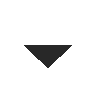
\includegraphics[height=0.8\baselineskip]{figures/collapse-symbol-1.eps} and 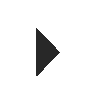
\includegraphics[height=0.8\baselineskip]{figures/collapse-symbol-2.eps} symbols at the beginning of the texts to toggle more detailed descriptions.



\begin{figure}[tp]
    \centering
    \setlength{\belowcaptionskip}{-10pt}
    \includegraphics[width=1\columnwidth]{figures/Movie-Actor-Jean-Pierre.eps}
    \caption{Case 1: Usage Scenario. (a) is the node-link diagram created with the Movie-J.P.M. graph (14 nodes and 25 links). (b) When the user hovers on a node, its related descriptions will be highlighted in (c).}
    \label{fig:Movie-Actor-Jean-Pierre}
\end{figure}